\documentclass[11pt,letterpaper]{article}

\usepackage[margin=1in]{geometry}
\usepackage{enumitem}
\usepackage{hyperref}
\usepackage{amsmath}
\usepackage{amssymb}
\usepackage{booktabs}
\usepackage{float}
\usepackage{listings}
\usepackage{xcolor}
\usepackage{tikz}
\usetikzlibrary{decorations.pathmorphing, decorations.pathreplacing, calc, arrows.meta}

\title{16.07 Dynamics Problem Set 6}
\author{Due Wednesday, November 18}
\date{}

% vector / matrix shorthands
\newcommand{\bw}{\boldsymbol{\omega}}
\newcommand{\Bw}{{}^{B}\boldsymbol{\omega}}
\newcommand{\bh}{\mathbf{h}}
\newcommand{\Nht}{{}^{N}\mathbf{h}}
\newcommand{\bJ}{\mathbf{J}}
\newcommand{\bA}{\mathbf{A}}
\newcommand{\ba}{\mathbf{a}}
\newcommand{\bq}{\mathbf{q}}
\newcommand{\bx}{\mathbf{x}}
\newcommand{\bu}{\mathbf{u}}
\newcommand{\bB}{\mathbf{B}}
\newcommand{\bM}{\mathbf{M}}
\newcommand{\br}{\mathbf{r}}
\newcommand{\bv}{\mathbf{v}}
\newcommand{\bd}{\mathbf{d}}
\newcommand{\bF}{\mathbf{F}}
\newcommand{\btau}{\boldsymbol{\tau}}
\newcommand{\bwr}{\mathbf{w}}
\newcommand{\Nr}{{}^{N}\mathbf{r}}
\newcommand{\Nrd}{{}^{N}\dot{\mathbf{r}}}
\newcommand{\BF}{{}^{B}\mathbf{F}}
\newcommand{\Btau}{{}^{B}\boldsymbol{\tau}}

\lstset{basicstyle=\ttfamily\small, columns=fullflexible, keepspaces=true,
    frame=single, rulecolor=\color{gray!60}, backgroundcolor=\color{gray!5},
    xleftmargin=0.5em, xrightmargin=0.5em, aboveskip=0.6em, belowskip=0.6em}

\begin{document}

\maketitle

\section*{Spacecraft Dynamics With Reaction Control Thrusters}

\begin{figure}[h]
\centering
% ---------------- Left panel: side view (x right, z up, y into the page) ----------------
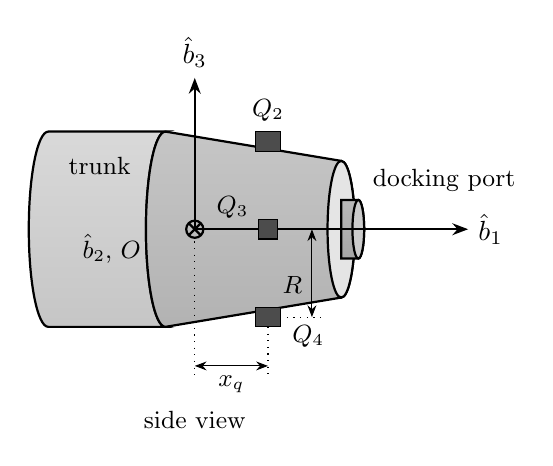
\begin{tikzpicture}[scale=0.62]
    % Units: meters. Body-frame origin O at the vehicle CoM.
    % Trunk (aft)
    % Drawn in slight perspective from the nose side, so circular sections appear as ellipses.
    \shadedraw[top color=gray!30, middle color=gray!3, bottom color=gray!45, draw=black, thick]
        (-3.0,2.0) -- (-0.6,2.0) arc[start angle=90, end angle=270, x radius=0.4, y radius=2.0]
        -- (-3.0,-2.0) arc[start angle=270, end angle=90, x radius=0.4, y radius=2.0] -- cycle;
    \node[font=\small] at (-1.95,1.3) {trunk};
    % Capsule (truncated cone)
    \shadedraw[top color=gray!45, middle color=gray!12, bottom color=gray!60, draw=black, thick]
        (-0.6,2.0) -- (3.0,1.4) arc[start angle=90, end angle=-90, x radius=0.28, y radius=1.4]
        -- (-0.6,-2.0) arc[start angle=270, end angle=90, x radius=0.4, y radius=2.0] -- cycle;
    % Nose face
    \filldraw[fill=gray!20, draw=black, thick] (3.0,0) ellipse[x radius=0.28, y radius=1.4];
    % Docking port at the nose
    \shadedraw[top color=gray!55, middle color=gray!25, bottom color=gray!70, draw=black, thick]
        (3.0,0.6) -- (3.35,0.6) arc[start angle=90, end angle=-90, x radius=0.12, y radius=0.6]
        -- (3.0,-0.6) -- cycle;
    \filldraw[fill=gray!40, draw=black, thick] (3.35,0) ellipse[x radius=0.12, y radius=0.6];
    \node[font=\small, anchor=west] at (3.45,1.0) {docking port};

    % Thruster pods Q2 (top, +z) and Q4 (bottom, -z) at station x_q
    \filldraw[fill=black!70, draw=black] (1.25,1.6) rectangle (1.75,2.0);
    \filldraw[fill=black!70, draw=black] (1.25,-2.0) rectangle (1.75,-1.6);
    \node[font=\small, above] at (1.5,2.0) {$Q_2$};
    \node[font=\small, anchor=west] at (1.8,-2.2) {$Q_4$};


    % Body axes at the CoM
    \draw[-{Stealth[length=2mm]}, thick] (0,0) -- (5.6,0) node[right] {$\hat b_1$};
    \draw[-{Stealth[length=2mm]}, thick] (0,0) -- (0,3.1) node[above] {$\hat b_3$};
    \draw[thick] (0,0) circle (5pt);
    \draw[thick] (-3.5pt,-3.5pt) -- (3.5pt,3.5pt);
    \draw[thick] (-3.5pt,3.5pt) -- (3.5pt,-3.5pt);
    \node[font=\small] at (-1.7,-0.4) {$\hat b_2$, $O$};

    % Thruster pod Q3 (-y, on the near side facing the viewer)
    \filldraw[fill=black!70, draw=black] (1.3,-0.2) rectangle (1.7,0.2);
    \node[font=\small, anchor=east] at (1.3,0.45) {$Q_3$};

    % Dimension: x_q
    \draw[dotted] (1.5,-2.0) -- (1.5,-3.0);
    \draw[dotted] (0,-0.25) -- (0,-3.0);
    \draw[{Stealth[length=1.5mm]}-{Stealth[length=1.5mm]}] (0,-2.8) -- (1.5,-2.8) node[midway, below, font=\small] {$x_q$};
    % Dimension: R
    \draw[{Stealth[length=1.5mm]}-{Stealth[length=1.5mm]}] (2.4,0) -- (2.4,-1.8);
    \node[font=\small, anchor=east] at (2.4,-1.15) {$R$};
    \draw[dotted] (1.75,-1.8) -- (2.6,-1.8);

    \node[font=\small] at (0,-3.9) {side view};
\end{tikzpicture}
\hspace{0.4cm}
% ---------------- Right panel: nose-on view (y right, z up, x out of the page) ----------------
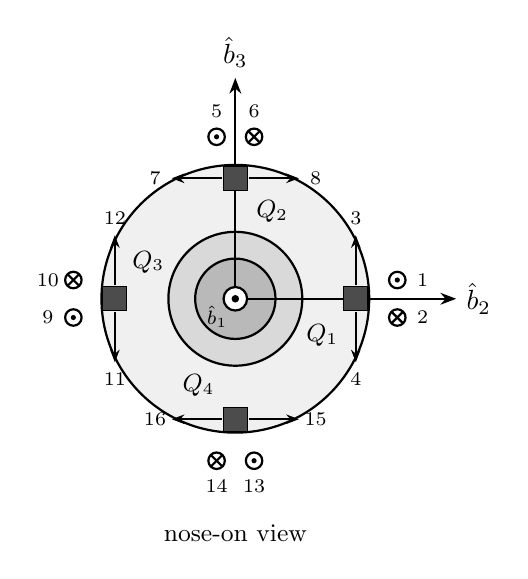
\begin{tikzpicture}[scale=0.85]
    \def\R{1.8}
    % Outlines: capsule base, nose, docking port
    \filldraw[fill=gray!12, draw=black, thick] (0,0) circle (2.0);
    \filldraw[fill=gray!30, draw=black, thick] (0,0) circle (1.0);
    \filldraw[fill=gray!55, draw=black, thick] (0,0) circle (0.6);

    % Body axes
    \draw[-{Stealth[length=2mm]}, thick] (0,0) -- (3.3,0) node[right] {$\hat b_2$};
    \draw[-{Stealth[length=2mm]}, thick] (0,0) -- (0,3.3) node[above] {$\hat b_3$};
    \filldraw[fill=white, thick] (0,0) circle (5pt);
    \fill (0,0) circle (1.6pt);
    \node[font=\scriptsize] at (-0.27,-0.27) {$\hat b_1$};


    % Quads
    \foreach \k in {1,...,4}{
        \pgfmathsetmacro{\ph}{90*(\k-1)}
        \pgfmathsetmacro{\cx}{\R*cos(\ph)}
        \pgfmathsetmacro{\cy}{\R*sin(\ph)}
        \pgfmathsetmacro{\tx}{-sin(\ph)}
        \pgfmathsetmacro{\ty}{cos(\ph)}
        \pgfmathsetmacro{\ex}{cos(\ph)}
        \pgfmathsetmacro{\ey}{sin(\ph)}
        \pgfmathtruncatemacro{\na}{4*\k-3}
        \pgfmathtruncatemacro{\nb}{4*\k-2}
        \pgfmathtruncatemacro{\nc}{4*\k-1}
        \pgfmathtruncatemacro{\nd}{4*\k}
        % pod
        \filldraw[fill=black!70, draw=black, rotate around={\ph:(\cx,\cy)}] ({\cx-0.18},{\cy-0.18}) rectangle ({\cx+0.18},{\cy+0.18});
        % tangential force arrows
        \draw[-{Stealth[length=1.6mm]}, thick] ({\cx+0.2*\tx},{\cy+0.2*\ty}) -- ({\cx+0.95*\tx},{\cy+0.95*\ty});
        \draw[-{Stealth[length=1.6mm]}, thick] ({\cx-0.2*\tx},{\cy-0.2*\ty}) -- ({\cx-0.95*\tx},{\cy-0.95*\ty});
        \node[font=\scriptsize] at ({\cx+1.2*\tx},{\cy+1.2*\ty}) {\nc};
        \node[font=\scriptsize] at ({\cx-1.2*\tx},{\cy-1.2*\ty}) {\nd};
        % axial force markers (out of page = +b1, into page = -b1)
        \coordinate (A) at ({\cx+0.62*\ex+0.28*\tx},{\cy+0.62*\ey+0.28*\ty});
        \coordinate (C) at ({\cx+0.62*\ex-0.28*\tx},{\cy+0.62*\ey-0.28*\ty});
        \filldraw[fill=white, thick] (A) circle (3.5pt);
        \fill (A) circle (1.1pt);
        \draw[thick] (C) circle (3.5pt);
        \draw[thick] ($(C)+(-2.4pt,-2.4pt)$) -- ($(C)+(2.4pt,2.4pt)$);
        \draw[thick] ($(C)+(-2.4pt,2.4pt)$) -- ($(C)+(2.4pt,-2.4pt)$);
        \node[font=\scriptsize] at ({\cx+1.0*\ex+0.28*\tx},{\cy+1.0*\ey+0.28*\ty}) {\na};
        \node[font=\scriptsize] at ({\cx+1.0*\ex-0.28*\tx},{\cy+1.0*\ey-0.28*\ty}) {\nb};
        % quad label
        \node[font=\small] at ({\cx-0.5*\ex-0.55*\tx},{\cy-0.5*\ey-0.55*\ty}) {$Q_{\k}$};
    }

    \node[font=\small] at (0,-3.5) {nose-on view};
\end{tikzpicture}
\\[0.5cm]
% ---------------- Bottom panel: schematic of quad Q3 (same orientation as the side view) ----------------
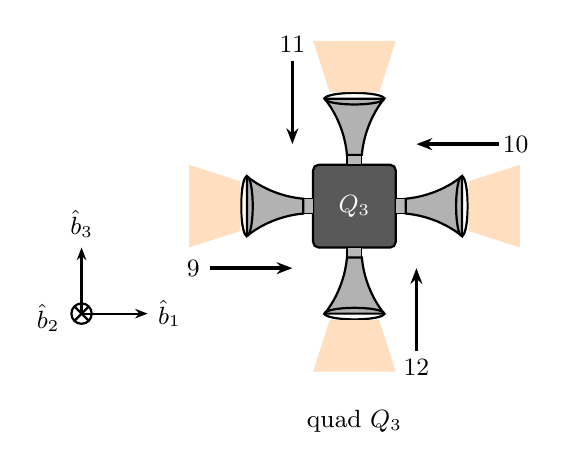
\begin{tikzpicture}[scale=1.05]
    % Pod body
    \filldraw[fill=black!65, draw=black, thick, rounded corners=2pt] (-0.5,-0.5) rectangle (0.5,0.5);
    \node[white, font=\small] at (0,0) {$Q_3$};
    % Four engine bells. Local frame: each bell opens along local +x (exhaust direction);
    % the force on the vehicle is along local -x. {rotation/thruster/label side}
    \foreach \rot/\num in {180/9, 0/10, 90/11, 270/12}{
        \begin{scope}[rotate=\rot]
            % throat
            \filldraw[fill=gray!55, draw=black] (0.5,-0.09) rectangle (0.62,0.09);
            % bell
            \shadedraw[top color=gray!60, middle color=gray!10, bottom color=gray!60, draw=black, thick, shading angle=\rot]
                (0.62,0.09) .. controls (0.85,0.11) and (1.1,0.2) .. (1.3,0.36)
                -- (1.3,-0.36) .. controls (1.1,-0.2) and (0.85,-0.11) .. (0.62,-0.09) -- cycle;
            \draw[thick] (1.3,0) ellipse[x radius=0.07, y radius=0.36];
            % exhaust plume
            \fill[orange!25] (1.38,0.3) -- (2.0,0.5) -- (2.0,-0.5) -- (1.38,-0.3) -- cycle;
            % force on the vehicle (opposite to the exhaust)
            \draw[-{Stealth[length=2mm]}, very thick] (1.75,0.75) -- (0.75,0.75);
            \node[font=\small] at (1.95,0.75) {\num};
        \end{scope}
    }
    % Axes
    \begin{scope}[shift={(-3.3,-1.3)}]
        \draw[-{Stealth[length=1.6mm]}, thick] (0,0) -- (0.8,0) node[right, font=\small] {$\hat b_1$};
        \draw[-{Stealth[length=1.6mm]}, thick] (0,0) -- (0,0.8) node[above, font=\small] {$\hat b_3$};
        \draw[thick] (0,0) circle (3.5pt);
        \draw[thick] (-2.4pt,-2.4pt) -- (2.4pt,2.4pt);
        \draw[thick] (-2.4pt,2.4pt) -- (2.4pt,-2.4pt);
        \node[font=\small, anchor=east] at (-0.15,-0.05) {$\hat b_2$};
    \end{scope}
    \node[font=\small] at (0,-2.6) {quad $Q_3$};
\end{tikzpicture}
\caption{Simplified Dragon-like spacecraft with 16 RCS thrusters arranged in four quads $Q_1,\dots,Q_4$. The body frame $B$ has its origin at the vehicle center of mass $O$, with $\hat b_1$ along the symmetry axis toward the docking port. Top left: side view ($\hat b_2$ into the page; $Q_1$ is hidden behind the vehicle). Top right: view looking at the nose ($\hat b_1$ out of the page). Bottom: schematic of quad $Q_3$ in the same orientation as the side view, showing its four engine bells; each thruster's exhaust leaves through its bell, and the arrow next to it shows the resulting force on the vehicle. Arrows and the $\odot$/$\otimes$ symbols show the direction of the force each thruster applies \emph{to the vehicle} (opposite to its exhaust), labeled with the thruster number. Drawings are not to scale.}
\label{fig:dragon}
\end{figure}

\noindent In this problem set, you'll build a full six-degree-of-freedom simulation of a spacecraft in low-Earth orbit, loosely modeled on SpaceX's Dragon. Dragon maneuvers using 16 Draco thrusters, grouped into four quads of four thrusters each. Each Draco produces about 400~N of thrust in vacuum. You'll derive how the thruster commands map into a force and torque on the vehicle, write the Newton--Euler equations of motion in manipulator form, compare two fixed-step integrators, and pose thruster allocation as an optimization problem.

We'll use the following notation and assumptions throughout:
\begin{itemize}
    \item $N$ is an Earth-centered inertial (ECI) frame. $B$ is the body frame shown in Fig.~\ref{fig:dragon}, with origin at the vehicle's center of mass $O$ and axes along its principal axes. As in Problem Sets 4 and 5, a left superscript denotes the frame in which a vector's components are expressed.
    \item Attitude is represented by a unit quaternion $\ba$, using the conventions from class and Problem Set 5, so the rotation matrix $\bA = \bA(\ba)$. \emph{Note the change of notation:} in Problem Sets 4 and 5 we called the rotation matrix $\mathbf{Q}$ and the quaternion $\mathbf{q}$. Here we'll call them $\bA$ and $\ba$ (for ``attitude''), so that we can use $\bq$ for the configuration vector in Part 2.
    \item $\Nr$ and $\Nrd$ are the position and velocity of the vehicle's center of mass relative to the center of the Earth, and $\Bw$ is the vehicle's angular velocity relative to $N$, expressed in the body frame.
    \item The Earth is assumed to be perfectly spherical with gravitational parameter $\mu = 3.986004418\times10^{14}$~m$^3$/s$^2$. There are no other external forces or torques.
    \item The vehicle is rigid and its mass and inertia are constant (we neglect the propellant consumed).
    \item Each thruster $i$ produces a force of magnitude $u_i$ along a fixed direction in the body, and can be throttled continuously over $0 \le u_i \le u_{\max}$. (Real Dracos are pulsed on and off, but a continuous throttle is a good model of their average effect.)
\end{itemize}
We'll work in SI units throughout.

\section*{Part 1: Vehicle Model and the Input Jacobian}

The vehicle's mass properties and thruster specifications are given in Table~\ref{tab:vehicle}. The mass is close to Crew Dragon's in-orbit mass with its trunk attached. The inertia matrix is an illustrative estimate, since SpaceX doesn't publish one.

Each quad is a pod of four thrusters, and we'll treat all four thrusters in a pod as acting at the pod's location. The pods all sit $x_q = 1.5$~m forward of $O$, at a distance $R = 1.8$~m from the $\hat b_1$ axis (Fig.~\ref{fig:dragon}). Quad $Q_k$ contains thrusters $4k-3$ through $4k$, numbered as in Fig.~\ref{fig:dragon}. The positions ${}^{B}\br_i$ of the thrusters relative to $O$, in body-frame components, are
\begin{align*}
{}^{B}\br_1 = {}^{B}\br_2 = {}^{B}\br_3 = {}^{B}\br_4 &= \begin{bmatrix} 1.5 & 1.8 & 0 \end{bmatrix}^T\text{ m} && (Q_1), \\
{}^{B}\br_5 = {}^{B}\br_6 = {}^{B}\br_7 = {}^{B}\br_8 &= \begin{bmatrix} 1.5 & 0 & 1.8 \end{bmatrix}^T\text{ m} && (Q_2), \\
{}^{B}\br_9 = {}^{B}\br_{10} = {}^{B}\br_{11} = {}^{B}\br_{12} &= \begin{bmatrix} 1.5 & -1.8 & 0 \end{bmatrix}^T\text{ m} && (Q_3), \\
{}^{B}\br_{13} = {}^{B}\br_{14} = {}^{B}\br_{15} = {}^{B}\br_{16} &= \begin{bmatrix} 1.5 & 0 & -1.8 \end{bmatrix}^T\text{ m} && (Q_4).
\end{align*}

\begin{table}[H]
\centering
\small
\begin{tabular}{lll}
\toprule
Quantity & Symbol & Value \\
\midrule
Mass & $m$ & $12{,}500$~kg \\
Inertia matrix about $O$, in $B$ & $\bJ$ & $\operatorname{diag}\left(22,\ 48,\ 52\right)\times10^{3}$~kg\,m$^2$ \\
Number of thrusters & & 16 (4 quads $\times$ 4) \\
Maximum thrust per thruster & $u_{\max}$ & 400~N \\
\bottomrule
\end{tabular}
\caption{Vehicle parameters.}
\label{tab:vehicle}
\end{table}

\begin{enumerate}[label=(\alph*)]
    \item \textbf{Thrust directions:} Using Fig.~\ref{fig:dragon}, find the unit vector ${}^{B}\bd_i$ along which each thruster's force vector points in the body frame. Write these in a table.

    \item \textbf{Input Jacobian:} Write the force and torque that thruster $i$ applies to the vehicle, in terms of $u_i$, ${}^{B}\br_i$, and ${}^{B}\bd_i$. The total \emph{wrench} (force and torque) on the vehicle in terms of the thrust commands $\bu = [u_1\;\cdots\;u_{16}]^T$ can be written in matrix form,
    \[
    {}^{B}\bwr = \begin{bmatrix} \BF \\ \Btau \end{bmatrix} = \bB\,\bu,
    \]
    where the $6\times16$ matrix $\bB$ is called the \emph{input Jacobian}. Write $\bB$ in terms of the ${}^{B}\br_i$ and ${}^{B}\bd_i$. Why is $\bB$ constant in the body frame?
\end{enumerate}

\section*{Part 2: Equations of Motion}

We'll write the translational dynamics in inertial (ECI) $N$-frame components, rather than in the body frame. Gravity takes its simplest form in $N$, but the thrust force, which is naturally expressed in $B$, must be rotated into $N$ using the attitude. The rotational dynamics, as in Problem Set 4, are written in body-frame components, where $\bJ$ is constant.

\begin{enumerate}[label=(\alph*)]
    \item \textbf{Newton--Euler equations:} Write Newton's 2nd law for the translational motion of the center of mass in inertial $N$-frame components, including both gravity and the thrust force $\BF$. Remember that the thrust force from Part 1 is expressed in $B$, so you'll have to rotate it. Then write Euler's equation for the rotational motion in $B$-frame components, using the thrust torque $\Btau$ from Part 1.

    \item \textbf{Manipulator form:} Define the configuration and velocity vectors
    \[
    \bq = \begin{bmatrix} \Nr \\ \ba \end{bmatrix} \in \mathbb{R}^7, \qquad
    \bv = \begin{bmatrix} \Nrd \\ \Bw \end{bmatrix} \in \mathbb{R}^6.
    \]
    Using the quaternion kinematics from class and Problem Set 5 (with $\bq$ there renamed $\ba$), write the kinematics in the form $\dot\bq = \mathbf{N}(\bq)\,\bv$, and give the $7\times6$ matrix $\mathbf{N}(\bq)$. Then write the dynamics in \emph{manipulator form},
    \[
    \bM(\bq)\,\dot\bv + \mathbf{c}(\bq,\bv) + \mathbf{g}(\bq) = \bB(\bq)\,\bu,
    \]
    where $\mathbf{c}(\bq,\bv) \in \mathbb{R}^6$ collects all of the velocity-dependent terms and $\mathbf{g}(\bq) \in \mathbb{R}^6$ collects the gravity terms. Write out $\bM$, $\mathbf{c}$, $\mathbf{g}$, and the $6\times16$ matrix $\bB(\bq)$ in terms of the input Jacobian $\bB$ from Part 1. Why is $\bB$ constant, while $\bB(\bq)$ is not?
\end{enumerate}

\section*{Part 3: Simulation}

So far, we've used adaptive integrators like \texttt{ode45} and \texttt{solve\_ivp}. A flight computer, however, usually runs at a fixed rate: it reads its sensors, computes thruster commands, and holds those commands constant until the next update. In this part, you'll simulate the vehicle with two simple fixed-step integrators running at 20~Hz, i.e., with time step $h = 0.05$~s. Writing $\bx_k = \bx(kh)$ and holding $\bu_k$ constant over each step, the two schemes are:
\begin{align*}
\text{Forward Euler:} \qquad & \bx_{k+1} = \bx_k + h\,\mathbf{f}(\bx_k, \bu_k), \\
\text{Explicit midpoint:} \qquad & \bx_{k+1} = \bx_k + h\,\mathbf{f}\!\left(\bx_k + \tfrac{h}{2}\,\mathbf{f}(\bx_k,\bu_k),\ \bu_k\right).
\end{align*}
Forward Euler is first-order accurate, and explicit midpoint (a 2nd-order Runge--Kutta method) is second-order accurate.

We'll start the vehicle in a circular orbit similar to that of the International Space Station (ISS), at an altitude of about 420~km and an inclination of $i = 51.64^\circ$. The initial conditions are
\[
\Nr(0) = \begin{bmatrix} r_0 \\ 0 \\ 0 \end{bmatrix}, \quad
\Nrd(0) = v_c\begin{bmatrix} 0 \\ \cos i \\ \sin i \end{bmatrix}, \quad
\ba(0) = \begin{bmatrix} 1 \\ 0 \\ 0 \\ 0 \end{bmatrix}, \quad
\Bw(0) = \begin{bmatrix} 1 \\ 0.5 \\ -0.5 \end{bmatrix}\text{ deg/s},
\]
where
\[
r_0 = 6{,}797{,}956.058\text{ m}, \qquad v_c = \sqrt{\mu/r_0} = 7{,}657.371391\text{ m/s}, \qquad \Nrd(0) = \begin{bmatrix} 0 \\ 4{,}752.168573 \\ 6{,}004.350962 \end{bmatrix}\text{ m/s}.
\]
All thrusters are off, $\bu = \mathbf{0}$. This orbit's period is exactly $P = 2\pi\sqrt{r_0^3/\mu} = 5{,}578.0$~s (about 93 minutes), so after one period the vehicle should return exactly to its starting position. Compute $v_c$ in your code from $\mu$ and $r_0$, rather than typing in the rounded value.

\begin{enumerate}[label=(\alph*)]
    \item \textbf{First-order ODE:} Define the 13-dimensional state vector $\bx = [\bq^T\;\,\bv^T]^T$ and write the full dynamics as a first-order vector ODE $\dot\bx = \mathbf{f}(\bx,\bu)$. Implement $\mathbf{f}$ as a function in MATLAB or Python, reusing your quaternion functions from Problem Set 5.

    \item \textbf{Integrators:} Implement one step of each scheme as a function that takes $\bx_k$, $\bu_k$, and $h$ and returns $\bx_{k+1}$. At the end of every step, renormalize the quaternion, $\ba \leftarrow \ba/\lVert\ba\rVert$, before returning $\bx_{k+1}$.

    \item \textbf{One orbit:} Using each scheme with $h = 0.05$~s, simulate exactly one orbital period, $K = P/h = 111{,}560$ steps. For each scheme, report:
    \begin{itemize}
        \item The orbital position error after one period, $\lVert\Nr(P) - \Nr(0)\rVert$.
        \item The relative error in the angular momentum after one period, $\lVert\Nht(P) - \Nht(0)\rVert/\lVert\Nht(0)\rVert$, where $\Nht = \bA(\ba)\,\bJ\,\Bw$.
    \end{itemize}

    \item \textbf{Comparison:}
    \begin{itemize}
        \item Which scheme is more accurate, and by roughly how much?
        \item Explicit midpoint evaluates $\mathbf{f}$ twice per step, so it costs about twice as much as forward Euler. To compare at equal cost, rerun forward Euler with $h = 0.025$~s (40~Hz, $K = 223{,}120$ steps) for one orbit. How does its position error compare with your 20~Hz midpoint result? Explain using the order of accuracy of each method.
        \item A docking port is about a meter across. Which of these integrators would you trust to simulate a rendezvous with the ISS?
    \end{itemize}
\end{enumerate}

\section*{Part 4: Thruster Allocation}

A spacecraft's guidance and control software typically decides what force and torque it wants, ${}^{B}\bwr_{\text{des}}$, and then has to choose thruster commands $\bu$ that produce it. This is called \emph{thruster allocation}. Since $\bB$ has many more columns than rows, there are infinitely many solutions to $\bB\bu = {}^{B}\bwr_{\text{des}}$, and we need a principled way to choose one.

\begin{enumerate}[label=(\alph*)]
    \item \textbf{Naive pseudoinverse:} Suppose we want a pure $+\hat b_2$ translation force of 200~N with no torque:
    \[
    {}^{B}\bwr_{\text{des}} = \begin{bmatrix} 0 & 200 & 0 & 0 & 0 & 0 \end{bmatrix}^T.
    \]
    Since $\bB$ is not square, compute $\bu = \bB^{+}\,{}^{B}\bwr_{\text{des}}$, where $\bB^{+}$ is the Moore--Penrose pseudoinverse (\texttt{pinv} in MATLAB or \texttt{numpy.linalg.pinv}). Verify that $\bB\bu = {}^{B}\bwr_{\text{des}}$. Can the thrusters actually produce this $\bu$? Why or why not? \emph{Hint: Can thrusters produce negative thrust?}

    \item \textbf{Thruster allocation as a QP:} We can fix this by posing allocation as a constrained optimization problem. Among all thrust commands that produce the desired wrench and respect the thruster limits, we'll choose the one with the least total ``effort,'' measured by $\lVert\bu\rVert^2$:
    \begin{equation*}
    \begin{aligned}
    \underset{\bu \in \mathbb{R}^{16}}{\text{minimize}} \quad & \tfrac12\,\bu^T\bu \\
    \text{subject to} \quad & \bB\,\bu = {}^{B}\bwr_{\text{des}}, \\
    & 0 \le u_i \le u_{\max}, \quad i = 1,\dots,16.
    \end{aligned}
    \end{equation*}
    This is a \emph{quadratic program} (QP): a quadratic objective with linear equality and inequality constraints. Because the objective is strictly convex and the constraints are linear, a feasible QP has a unique global minimum that can be found reliably and quickly.
    
    Solving a QP like this takes only a few lines of code with a convex optimization package. In MATLAB, using CVX (\url{https://github.com/cvxr/CVX}):
\begin{lstlisting}[language=Matlab]
cvx_begin quiet
    variable u(16)
    minimize( 0.5 * sum_square(u) )
    subject to
        B * u == w_des;
        0 <= u <= u_max;
cvx_end
\end{lstlisting}
    In Python, using CVXPY (\texttt{pip install cvxpy}):
\begin{lstlisting}[language=Python]
import cvxpy as cp

u = cp.Variable(16)
objective = cp.Minimize(0.5 * cp.sum_squares(u))
constraints = [B @ u == w_des, u >= 0, u <= u_max]
prob = cp.Problem(objective, constraints)
prob.solve()
print(prob.status, u.value)
\end{lstlisting}
    Use this code to solve the QP for two desired wrenches:
    \begin{itemize}
        \item The pure $+\hat b_2$ force of 200~N from part (a).
        \item A combined 300~N force along $+\hat b_1$ and a 100~N\,m roll torque about $+\hat b_1$.
    \end{itemize}
    For each, report $\bu$, verify that $\bB\bu = {}^{B}\bwr_{\text{des}}$ and that all constraints are satisfied, and explain physically which thrusters fire and why. For the first wrench, how is the QP solution related to the pseudoinverse solution from part (a)? \emph{Hint: Look at each opposed pair of thrusters.}
\end{enumerate}

\end{document}
